\section{Cuestiones a resolver}
A continuación se detalla una serie de cuestiones planteadas por la cátedra.

\subsection{Posición de esteganografiado}
\begin{displayquote}
Para la implementación del programa stegobmp se pide que la ocultación comience en el
primer componente del primer pixel. ¿Sería mejor empezar en otra ubicación? ¿Por qué? 
\end{displayquote}

Al realizar siempre la oculatción en el primer píxel, existe la posibilidad de notar las alteraciones en el BMP para LSB1, LSB4 y LSBE en las porciones de color blanco en la parte inferior de la imagen. El hecho es evidenciable a simple vista en la imagen "lado.bmp" provista por la cátedra, que aparenta tener una ligera sombra de "ruido" o "lluvia" hasta determinada altura. Esto hace que una persona pueda sospechar del contenido de los archivos.

Alterar el header es inviable. La ventaja de ocultar desde el comienzo del bitmap (es decir, luego del header) es que se logra un máximo de aprovechamiento del archivo.

\subsection{Ocultamiento en una componente puntual}
\begin{displayquote}
¿Qué ventajas podría tener ocultar siempre en una misma componente? Por ejemplo, siempre
en el bit menos significativo de la componente azul.
\end{displayquote}

La principal ventaja es que se reduce el nivel de alteración del archivo, lo que dificulta un poco más el análisis estadístico.

\subsection{Comparativa entre sistemas LS*}
\begin{displayquote}
Esteganografiar un mismo archivo en un .bmp con cada uno de los tres algoritmos, y comparar
los resultados obtenidos. Hacer un cuadro comparativo de los tres algoritmos estableciendo
ventajas y desventajas.
\end{displayquote}

Al realizar un esteganografiado 'pom.xml' (disponible en el repositorio) en un archivo 'lado.bmp' provisto por la cátedra y sin contenido oculto previo, se puede observar para los distintos algoritmos lo siguiente:

\begin{table}[H]
\centering
\caption{Comparativa de Sistemas LSB}
\label{comparativa-lsb}
\begin{tabular}{l|l|l|l}
\textbf{Ventaja}          & \textbf{LSB1} & \textbf{LSB4}  & \textbf{LSBE}    \\ \hline \hline
Tiempo de ejecución       & Medio         & Alto           & Bajo             \\  \hline
Alteración visible al ojo & Media a baja  & Alta (ruidosa) & Imperceptible    \\  \hline
Capacidad de ocultamiento & Media (1:8)   & Alta (1:2)     & Variable (baja)  \\  \hline
Depende del bmp portador  & Tamaño fijo   & Tamaño fijo    & Sí, muy variable \\  \hline
\end{tabular}
\end{table}

Por detalles de implementación, la copia a buffers muy pequeños en LSB4 hace que sea el más lento. LSB1 es un poco más rápido porque el tamaño de buffer es cuatro veces mayor. LSBE no usa el mismo mecanismo, por lo cual no se ve impactado del mismo modo.

De los tres sistemas, el más evidente al ojo es LSB4, ya que altera más bytes del portador. Asimismo, es el que más capacidad de almacenaje tiene, que sólo depende del tamaño de la imagen y no del contenido. De manera similar, LSB1 altera los bytes de manera menos evidente a costa de la capacidad de ocultamiento. LSBE es imperceptible, pero a costa de depender tanto del tamaño de la imagen como del contenido.

\subsection{Esteganografiado de la extensión}

\begin{displayquote}
Para la implementación del programa stegobmp se pide que la extensión del archivo se oculte
después del contenido completo del archivo. ¿por qué no conviene ponerla al comienzo,
después del tamaño de archivo?
\end{displayquote}

Si se serializa al comienzo, luego del tamaño del payload, es trivial detectar si existe esteganografía con sólo leer unos pocos bytes, y detectar si está cifrado o no. Se puede generar una máscara estática sobre los bytes del archivo para detectar la presencia del caracter esteganografiado ".", con lo que se puede extraer la extensión para LSB1 y LSB4, y de manera similar se puede realizar para LSBE. Esto nos da una señal inequívoca de qué sistema se emplea: si encontramos dicha marca entonces el archivo oculto no estará cifrado.

Si el archivo estuviera cifrado, se tiene una serie de bytes al comienzo por cifrar que no cambian. Dado que el IV depende de la clave y no se le puso sal, que se sugirió el uso de MD5 (roto), y que el conjunto de extensiones es pequeño, se introduce una reducción considerable en el espacio de búsqueda de claves; realizar un ataque de fuerza bruta sobre los primeros bytes es factible.

\subsection{Modo de análisis de archivos provistos}
\begin{displayquote}
Explicar detalladamente el procedimiento realizado para descubrir qué se había ocultado en
cada archivo y de qué modo.
\end{displayquote}

El análisis se realiza en primera instancia mediante la herramienta \texttt{stegobmp} en Guess Mode (implementado para realizar aproximaciones iniciales rápidas). El mismo realiza un análisis de fuerza bruta sobre el sistema de esteganografía empleado, usando tanto el tamaño como la extensión a modo de pistas.

Para aquellos archivos con resultados negativos ante el proceso anterior, se realiza un dump de  strings usando la herramienta \texttt{strings} de Unix. En el ejemplo provisto por la c\'atedra es f\'acil encontrar la clave al final de l archivo. Si no fuera as\'i, al contenido se le hace un grep buscando palabras disponibles en un diccionario (se puede encontrar un diccionario de palabras en \texttt{/usr/share/dict/words}).

Si el resultado anterior descubre palabras, se emplean como posibles passwords de los archivos que no arrojen resultados ante ninguno de los dos m\'etodos previamente mencionados, y para el archivo donde fue encontrada esa clave. El m\'etodo utilizado es nuevamente el Guess Mode.

\subsection{Contenido de los archivos con secretos}
\begin{displayquote}
¿Qué se encontró en cada archivo?
\end{displayquote}

La c\'atedra provee para el Grupo 12 cuatro archivos con las siguientes caracter\'isticas:

\subsubsection{\texttt{montevideo.bmp}}
El análisis del archivo en modo guess sin password no arroja resultados concluyentes. Ni la extensión ni el tamaño del archivo son válidos para cada sistema.

Se procede a utilizar el binario strings. Arroja, sorprendentemente, el resultado de:
\texttt{h4la password es exitoso} al final del archivo. Ninguna combinaci\'on arroja resultados concluyentes. Se asume que el archivo no tiene m\'as datos pasibles de criptoan\'alisis por ahora.

\subsubsection{\texttt{silence.bmp}}
El resultado inicial del Guess Mode sin password arroja lo siguiente:

\begin{lstlisting}
Guessing if silence.bmp can be decoded with LSB4Splitter
- silence.bmp seems to be a .png encoded with LSB4
Guessing if silence.bmp can be decoded with LSB1Splitter
- Hmm, nope.
Guessing if silence.bmp can be decoded with LSBESplitter
- Hmm, nope.
\end{lstlisting}

Se renombra la salida para que tenga extensi\'on png y se aprecia una imagen un juego clon de Buscaminas:

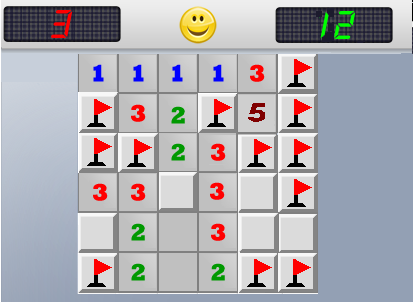
\includegraphics[width = 140mm]{silence_out.png}

Se concluye con alto grado de certidumbre que el archivo silence.bmp contiene un .png que fue esteganografiado con LSB4 y sin password.

\subsubsection{\texttt{quito.bmp}}
Un análisis inicial del archivo con Guess Mode revela la siguiente información:

\begin{lstlisting}
Guessing if quito.bmp can be decoded with LSB4Splitter
- Hmm, nope.
Guessing if quito.bmp can be decoded with LSB1Splitter
- quito.bmp seems to be a .wmv encoded with LSB1
Guessing if quito.bmp can be decoded with LSBESplitter
- Hmm, nope.
\end{lstlisting}

El análisis inicial nos hace sospechar de un .wmv, por lo que se renombra el resultado con tal extensión. Sin embargo, el archivo no es reconocido por su cabecera. El mismo comienza con 13F44B79, pero se espera 3026B27 según esta lista: \href{https://en.wikipedia.org/wiki/List_of_file_signatures}.

Procedemos a usar la password encontrada (exitoso) en \texttt{montevideo.bmp}:
\begin{lstlisting}
Guessing if quito.bmp can be decoded with LSB1Splitter + decoder aes192 cbc
- quito.bmp seems to be a .wmv encoded with LSB1
\end{lstlisting}

\subsubsection{\texttt{lado.bmp}}
El resultado inicial del Guess Mode sin password arroja lo siguiente:

\begin{lstlisting}
Guessing if lado.bmp can be decoded with LSB4Splitter
- Hmm, nope.
Guessing if lado.bmp can be decoded with LSB1Splitter
- Extension does not seem to be valid
Guessing if lado.bmp can be decoded with LSBESplitter
- lado.bmp seems to be a .pdf encoded with LSBE
\end{lstlisting}

El resultado es un .pdf que contiene la frase:
\begin{lstlisting}
al .png cambiarle la extension por .zip y descomprimir
\end{lstlisting}

\subsection{Ocultamiento de otros mensajes}
\begin{displayquote}
Algunos mensajes ocultos tenían, a su vez, otros mensajes ocultos. Indica cuál era ese mensaje
y cómo se había ocultado.
\end{displayquote}

El mensaje oculto dentro de otro está en \texttt{silence.bmp} y el resultado es un .zip.

El mismo se descubrió en base a otro archivo oculto extraído de \texttt{lado.bmp} que contiene la frase:
\begin{lstlisting}
al .png cambiarle la extension por .zip y descomprimir
\end{lstlisting}

Al zip se le ejecuta el comando 'unzip' de mac. El resultado es un archivo sol9.txt con el siguiente texto:

\begin{lstlisting}
cada mina es un 1.
cada fila forma una letra.
Los ascii de las letras empiezan todos en 01.
Asi encontraras el algoritmo que tiene clave de 192 bits y el modo
La password esta en otro archivo
Con algoritmo, modo y password hay un .wmv encriptado y oculto.
\end{lstlisting}

Se resuelve el juego (que est\'a incompleto) y la secuencia da:

\begin{lstlisting}
01000001
01100101
01110011

01000011
01100010
01100011
\end{lstlisting}

Que traduce a Aes Cbc de 192.

Se ejecuta con password 'exitoso' el stegobmp.
Guessing if quito.bmp can be decoded with LSB1Splitter + decoder aes192 cbc
- quito.bmp seems to be a .wmv encoded with LSB1

Se obtiene un video data.wmv.

\subsection{Ocultamiento del video}
\begin{displayquote}
Uno de los archivos ocultos era una porción de un video, donde se ve ejemplificado una manera
de ocultar información ¿cuál fue el portador?
\end{displayquote}

El portador fue \texttt{quito.bmp}.

El audio dice:
'Hay que ser cerdo para cortar con alguien por e-mail'

'Ya, como que hay un protocolo aceptable para partirle el coraz\'on a alguien... Eh, un segundo, qu\'e raro... Este archivo es m\'as grande de lo que deber\'ia, lo que significa que hay alg\'un error de compresi\'on.'

'O nuestro agente ocult\'o datos en el archivo.'


\subsection{Método NoLSB}
\begin{displayquote}
¿De qué se trató el método de estenografiado que no era LSB? ¿Es un método eficaz? ¿Por qué?
\end{displayquote}

El método fue simplemente agregar al final un texto plano a \texttt{montevideo.bmp}. El mismo fue fácil de encontrar ya que simplemente con un editor hexadecimal se puede ver. Es vulnerable a búsqueda de texto plano.

\subsection{Mejoras y propuestas}

\begin{displayquote}
¿Qué mejoras o futuras extensiones harías al programa stegobmp? 
\end{displayquote}

\subsubsection{Guess Mode}

Se propone, como se encuentra implementado, el modo "guess", que verifica mediante fuerza bruta el sistema utilizado para archivos esteganografiados no cifrados usando la extensión y verificación de tamaño. De obtenerse tamaños negativos o mayores de lo que puede sostener el archivo portador, éstos son descartados rápidamente. Si el tamaño tiene sentido, se verifica que la extensión tenga caracteres válidos (comience por punto, tenga caracteres legibles válidos de directorio y termine en cero) y que tenga un tamaño razonable.

El mismo sistema se emplea para archivos cifrados cuando se pasa la clave. Se ignora tanto el modo como el algoritmo y se saca el contenido por fuerza bruta.

\subsubsection{Bulk Report Mode}

Se aconseja que la funcionalidad de Guess Mode sea extendida para proveer un "Bulk Report Mode", que verifique todos los archivos BMP de un directorio y produzca un reporte para cada uno, junto con el archivo oculto (de encontrarse y tener un tamaño razonable límite).


\subsubsection{Cambio de posición de ocultamiento}

Se propone el siguiente modo: luego de ocultar los primeros cuatro bytes de tamaño (en Big Endian), insertar un número variable de bytes al azar en el rango 1 a 255 como padding hasta alcanzar como máximo N - 1 bytes ocultables (donde N es el payload esteganografiable, que sin contraseña es |archivo| + |extensión con punto y byte '0'| al final). Usar el byte '0' como marca, y colocar el payload. Continuar agregando bytes al azar hasta completar el archivo. Es decir, se emplea el bitmap entero, generando un nivel de ruido similar en todas las secciones del BMP.

\subsubsection{API de Streams}
Es posible convertir el sistema en dos clases wrappers de Input y Output streams. Esto permite agregar la funcionalidad de esteganografía a cualquier programa que quiera emplearla de modo transparente. Es destacable que la implementación puede soportar canales asincrónicos con mínimas modificaciones.


\subsubsection{Cifrado asimétrico}

Se puede cifrar una clave simétrica (de archivo, similar a lo que sería una de sesión) con una asimétrica. Las ventajas son:
\begin{itemize}
\item Sólo el receptor del mensaje puede leer su contenido real.
\item Cualquier persona con la llave pública puede ocultar un archivo, pero no leerlo.
\item Se puede agregar una firma para validar que el mensaje dentro del archivo es de una fuente confiable.
\end{itemize}